\documentclass{scrartcl}
\usepackage[utf8]{inputenc}
\usepackage{graphicx}%GRaphiken
\usepackage{tabularx}%Tabellen!
\usepackage[english]{babel}% Zeilentrennung besser
\usepackage{url}% Urls besser
\usepackage{textcomp}% Sonderzeichen
\usepackage{amsmath}%maths / equations
\usepackage{helvet}% Schrift Helvetica
% \usepackage[helvet]{sfmath}% Helvet also in Math modes
% \renewcommand\familydefault{\sfdefault}
\usepackage{sansmath} % sans in math
\usepackage[]{color}
\usepackage{todonotes}
\usepackage[
	left=3cm,
	right=2cm,
	top=1.5cm,
	bottom=1cm
	,
	includeheadfoot
	]{geometry}														% Satzspiegel
\usepackage[
	round,	%(defaultage in the main file and \input ) for round parentheses;
	%square,	% for square brackets;
	%curly,	% for curly braces;
	%angle,	% for angle brackets;
	colon,	% (default) to separate multiple citations with colons;
	%comma,	% to use commas as separaters;
	authoryear,% (default) for author-year citations;
	%numbers,	% for numerical citations;
	%super,	% for superscripted numerical citations, as in Nature;
	sort,		% orders multiple citations into the sequence in which they appear in the list of 				references;
	%sort&compress,    % as sort but in addition multiple numerical citations
                   % are compressed if possible (as 3-6, 15);
	%longnamesfirst,  % makes the first citation of any reference the equivalent of
                   % the starred variant (full author list) and subsequent citations
                   %normal (abbreviated list);
	%sectionbib,      % redefines \thebibliography to issue \section* instead of \chapter*;
                   % valid only for classes with a \chapter command;
                   % to be used with the chapterbib package;
	%nonamebreak,     % keeps all the authors names in a citation on one line;
                   %causes overfull hboxes but helps with some hyperref problems.
]{natbib}											    			% Literaturverzeichnis
\usepackage{scrhack}   % kills \float@addtolists!  warning
\usepackage[pdfpagelabels,plainpages=false, pageanchor=false]{hyperref}	


%% andere Einstellungen
\linespread{1.5}% 1.5 Zeilenabstand			
\graphicspath{{fig/}}                     % path to graphics


%% ----------------------------------------------------------------------------
\title{Ecotoxicology is not normal.}
\subtitle{How the use of proper statistical models can increase statistical power in ecotoxicological experiments.}
\author{Eduard Szöcs, Ralf B. Schäfer}
\date{\today}



%% ----------------------------------------------------------------------------
\begin{document}
\maketitle

\section*{Abstract}


%% --------------------------------
\section{Introduction}
In environmental risk assessments (ERA) statistical tests play an important role to evaluate the effects of pesticides. 
Despite criticism (e.g. \citet{landis_well_2011}) statistics like the No Observed Effect Concentration (NOEC) are still regularly used to report results experiments \citep{jager_bad_2012}. 
A critical issue of reporting a NOEC is the statistical power in the underlying experiments, i.e. the ability to detect an effect.

Ecotoxicologists perform various kinds of experiments yielding to different types of data, potentially with very low samples sizes. 
Examples are: animal counts in mesocosm experiments (positive, integer valued, discrete data), proportions of surviving animals (discrete, bonded between 0 and 1) or biomass in growth experiments (strictly positive data).

Such data are usually analysed by using methods assuming normal distributed data, although these types are inherently not normally distributed. 
In order to approximate the normality and variance homogeneity assumptions data is usually transformed.
It is advised that survival data can be transformed using an arcsine square root transformation \citep{oecd_current_2006, newman_quantitative_2012}. 
For count data from mesocosm experiments a log(Ax + 1) transformation is usually used, where the constant A is either chosen arbitrarily or following the recommendation of \citet{van_den_brink_impact_2000} Ax to be 2 for the lowest abundance value (x) greater than zero. 
Note, that there has been little evaluation and advice for the practitioners which transformations to use.
If the transformed data does not meet the normality assumptions, usually non-parametric tests are applied \citep{wang_making_2011}.

Generalized linear models (GLM) are a third possibility to analyse such not normally distributed data \citep{nelder_generalized_1972}.
GLMs can handle various types of data distributions, e.g. Poisson or negative binomial (for count data) or binomial (for discrete proportions); the normal distribution being a special case of GLMs.
Despite that GLMs were available more than 40 years now, ecotoxicologists do not regularly make use of them.

Recently studies concluded that data transformations should be avoided and GLMs be used as they have better statistical properties (\emph{Do not log-transform count data}, \citep{ohara_not_2010}; \emph{The arcsine is asinine}, \citep{warton_arcsine_2011}).

We first give two motivating examples showing that different methods may lead to different conclusions. 
% Then review what types of analysis are used by ecotoxicologists.
Then we compare these three types of methods (transformation and normality assumption, GLM, non-parametric tests) using simulations.


\section{Motivating examples}
\subsection{Count data}
\citet{brock_minimum_2014} provides a typical example data from a mesocosm study of mayfly larvae counts on artificial substrate samplers at one sampling day (Figure \ref{fig:example}). 
18 mesocosms have been sampled, with 6 treatments (Control, n = 4; 0.1 mg/L, 0.3mg/L, 1mg/l, 3mg/L, n = 3; 10 mg/L, n = 2).
We will use this data to demonstrate the differences between transformations, different GLMs and a non-parametric approach.

\subsubsection{The linear model}
To fit the standard linear model, we first transform the counts following \citet{van_den_brink_impact_2000}:
$$\begin{aligned}
  Y^T_i = log(AY + 1) \label{eqn:trans}
\end{aligned}$$
, where $Y$ is the measured abundance, $Y^T$ the transformed abundance and A = 5.5 (the lowest abundance value in the dataset is 11).

We fit the well known linear model:
$$\begin{aligned}
  Y^T &\sim N(\mu, \sigma^2) \nonumber \\
  var(Y^T) &= \sigma^2 \label{eqn:normal} \\
  Y^T &= \alpha + \beta X \nonumber
\end{aligned}$$
This model assumes a normal distributed response with constant variance ($\sigma$).
Note, that we it parametrised as contrast ($\beta X$) to the control group ($\alpha$) so that the LOEC can be directly deduced from the estimates of $\beta$.


\subsubsection{Generalized Linear Models}
GLMs are the extension of the normal model, by allowing other distributions of the response variable.
Instead of transforming the response variable the counts could be directly modelled by a Poisson distribution:

$$\begin{aligned}
  Y &\sim P(\lambda) \nonumber \\
  log~(\lambda) &= \mu \label{eqn:pois} \\
  \mu &= \alpha + \beta X \nonumber \\
  var(Y) &= \lambda \nonumber
\end{aligned}$$

Again, this model is parametrised as contrast to the control group. 
The expected value of Y ($\lambda$) are linked with a log-function to the predictors, to avoid negative fitted values. 
The Poisson distribution assumes that the mean and the variance are equal - a assumption that is rarely met with ecological data which is typically characterized by greater variance (overdispersion).
To overcome this problem a quasi-Poisson distribution could be used which introduces an additional overdispersion parameter ($\Theta$):
$$\begin{aligned}
  Y &\sim P(\lambda, \Theta) \label{eqn:quasi} \\
  % log~\lambda &= \mu \label{eqn:quasi} \\
  % \mu &= \alpha + \beta X \nonumber \\
  var(Y) &= \Theta \lambda  \nonumber
\end{aligned}$$

Another possibility to deal with overdispersion is to use a negative binomial distribution

$$\begin{aligned}
  Y &\sim NB(\lambda, \kappa) \label{eqn:negbin}  \\
  % log~\lambda &= \mu \label{eqn:negbin} \\
  % \mu &= \alpha + \beta X \nonumber \\
  var(Y) &= \lambda + \kappa \lambda^2 \nonumber
\end{aligned}$$

Note, that the quasi-Poisson model assumes a linear mean-variance relationship, whereas the negative binomial model a quadratic relationship.
The above described models are most commonly used in ecology, although other models for count data are possible, like the negative binomial with a linear mean variance relationship (also known as NB1) and the poisson inverse gaussian \citep{hilbe_modeling_2014}.


\subsubsection{Hypothesis testing}

We could test different hypotheses, (i) if is there any effect of the treatment and (i) test single treatments/parameters to determine the LOEC.
We used F-tests for the linear and quasi-Poisson models and Likelihood-Ratio (LR) tests for Poisson and Negative binomial models to test if there is any treatment related effect.
To assess the LOEC we used Dunnett contrasts with Wald t tests (normal and quasi-poisson) and Wald Z tests (Poisson and negative binomial) following general recommendations \citep{bolker_generalized_2009}. 
Moreover, we used parametric bootstrap (we generated 2000 bootstrap samples) to assess the LR and parameters in the negative binomial model \citep{faraway_extending_2006}.
For comparison, we also performed the commonly used non-parametric Kruskal-Wallis test and pairwise Wilcoxon test on untransformed data.
P-values from multiple comparisons where adjusted using the method of \citet{holm_simple_1979}.


\subsubsection{Results}
F-test of the linear model  (F = 2.57, p = 0.084) and the quasi-Poisson model (F = 2.90, p = 0.061) as well as Kruskal-Wallis test (p = 0.145) did not indicate any treatment related effects.
The LR test of the negative binomial model indicated a treatment related effect (LR = 13.99, p = 0.016), whereas parametric bootstrap did not (p = 0.058).
Because of overdispersion the Poisson model did not fit to the data and inferences are not valid.

All methods resulted in similar predicted values except the normal model predicting always lower abundances (Figure \ref{fig:example}). 
Confidence intervals (CI) where most narrow for the negative binomial model and widest for quasi-Poisson - especially at lower estimated abundances.
Accordingly, the determined LOECs differed (Normal: 3 mg/L, quasi-Poisson: \textgreater 10mg/L, negative binomial (Wald Z and bootstrap) : 0.3 mg/L).

\begin{figure}
  \centering
  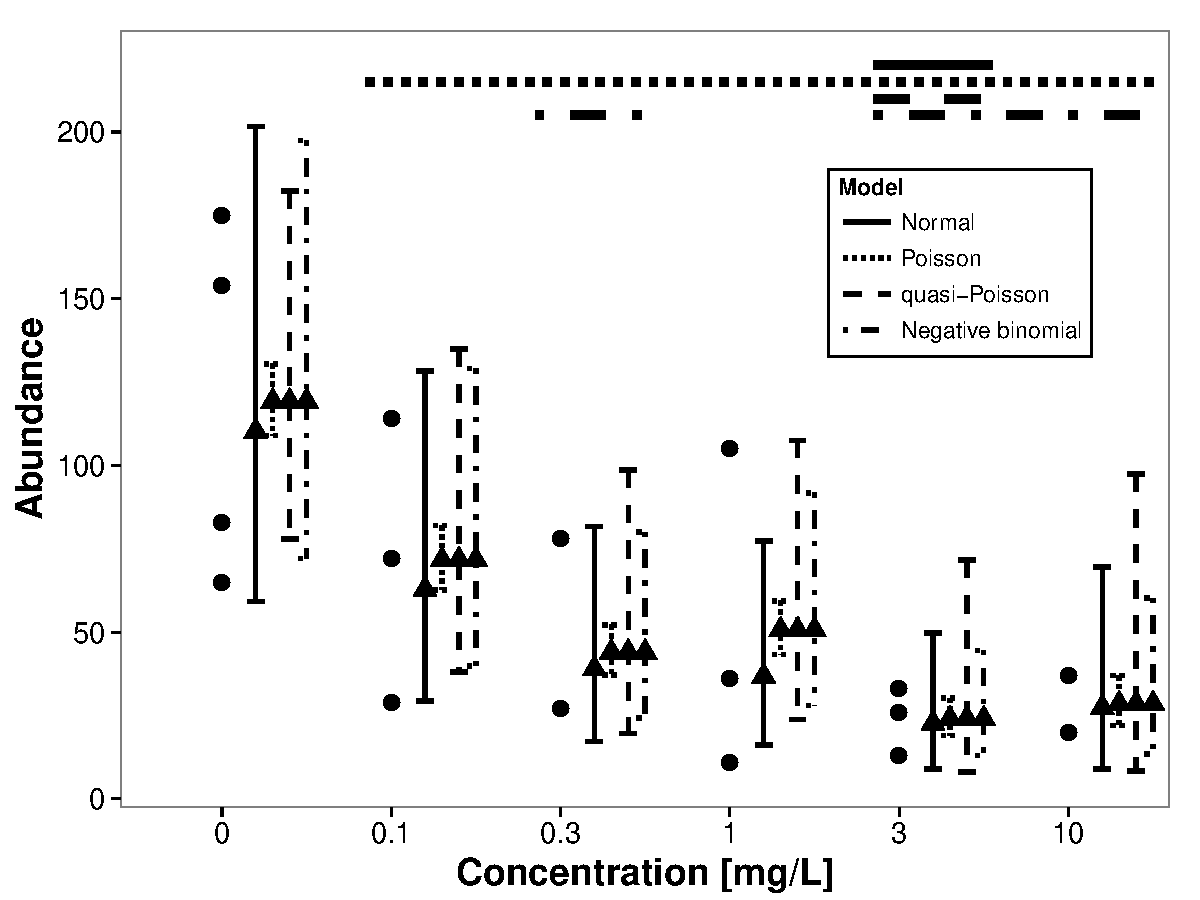
\includegraphics[width = 0.8\textwidth]{example.pdf}
  \caption{Data from \citet{brock_minimum_2014} (boxes + black points) and estimates + 95\% Wald Z or t Confidence intervals from the fitted models (vertical lines). 
  Bars above indicate treatments statistically significant different from the control group (Dunnett contrasts).}
  \label{fig:example}
\end{figure}

\subsection{Binomial data}
\citet{weber_short-term_1989} provides fathead minnow \textit{Pimephales promelas} larval survival data after sodium pentachlorophenol (NaPCP) exposure.
This data was also analysed in \citet{newman_quantitative_2012}.
At six NaPCP concentrations (0, 32, 64, 128, 256, 512 $\mu g / L$) with 4 replications ten fish were exposed and proportions of total number alive at the end reported.

\subsubsection{The linear model after transformation}
To accommodate the assumption for the standard linear model the EPA suggests a arcsine square root transformation for such kind of data \cite{epa_methods_2002}:

$$\begin{aligned}
  y^T = 
  \begin{cases}  
    arcsin(1) - arcsin(\sqrt{\frac{1}{4n}}) & \text{if}\ y = 1 \\
    arcsin(\sqrt{\frac{1}{4n}}) & \text{if}\ y = 0 \\
    arcsin(\sqrt{y}) & otherwise
  \end{cases}
\end{aligned}$$

, where $y^T$ are the transformed proportions and n is the number of exposed animals.
The transformed proportions are then analysed using the standard linear model (see above).

\subsubsection{Generalized Linear Models}

Data of type \emph{x out of n} are typically modelled by a binomial distribution with parameter n and $\pi$:

$$\begin{aligned}
  Y &\sim Bin(n, \pi,) \nonumber \\
  logit~(\pi) &= \alpha + \beta X \nonumber \label{eqn:bin} \\
  var(Y) &=  \pi (1 - \pi) / n \nonumber
\end{aligned}$$

, with n = number of exposed animals and $\pi$ is the probability of survival.
The variance of binomial proportion is a quadratic function of the mean.


\subsubsection{Results}
For this dataset, both methods yielded to same inferences:
The global tests of both methods indicated a strong effect of NaPCP on larval survival (linear model: F = 13.31, p \textless 0.001; GLM: $\chi^2$ = 64.79, p \textless 0.001).
Moreover, both methods identified the highest concentration ($521~\mu g / L$) as LOEC. 
The coefficients of the binomial model are directly interpretable as change in the odds ratio, whereas this is not possible with the transformed data.




%% --------------------------------
% \section{Review}
% The example above shows that different models and methods may lead to different conclusions.
% We now look at methods that are currently used by ecotoxicologists.



\section{Simulations}
We used simulations to compare the methods described above to analyse count and binomial data.
Methods were compare in terms of Type I error (maintain a significance level of 0.05 when there is no effect) and power (detect an effect when it is present). 
We fitted the models and tested hypotheses on the simulated data as described in the motivating example.

All simulations were done in R (Version 3.1.2) on a 64-bit Linux machine with 8 GB and 2.2 GHz.
Exemplary analysis of data in the motivating example can be found in the supplement.
Source code for the simulations is available online at \url{https://github.com/EDiLD/usetheglm}. 

\subsection{Count data}
\subsubsection{Methods}
We simulated count data that mimics count data encountered in mesocosm experiments, with five treatments (T1 - T5) and one control group (C) as in the motivating example. 

Counts were drawn from a negative binomial distribution with slight over dispersion (dispersion parameter for all treatments: $\kappa = 3.91$).
We simulated datasets with different number of replicates (N = \{3, 6, 9\}) and different abundances in control treatments ($\mu_\text{\tiny C}$ = \{2, 4, 8, 16, 32, 64, 128\}). 
For each combination we generated 100 datasets.
For power estimation mean abundance in treatments T2 - T5 was reduced to half of control and T1 ($\mu_\text{\tiny T2}~=~...~=~\mu_\text{\tiny T5}~=~0.5~\mu_\text{\tiny C} = 0.5~\mu_\text{\tiny T1}$), resulting to a theoretical LOEC at T2.
For Type I error estimation mean abundance was kept equal between all groups.


\subsubsection{Results}
For our simulation design (reduction in abundance by 50\%) a sample size of n = 9 was needed to achieve a power greater then 80\%.
Test of treatment effect for the negative binomial GLM (with LRT) showed an increased Type I error. However, this decreased to an acceptable limit with increasing sample sizes.
The linear model on transformed data, quasi-Poisson GLM and negative binomial GLM (with bootstrap) maintained an appropriate Type I error, with quasi-Poisson having greatest power (Figure \ref{fig:p_glob_c}).
The Kruskal-Wallis test showed least power, with low Type I error at small sample sizes.
For small sample sizes (n = {3, 6}) and low abundances ($\mu_C$ = {2, 4}) many of the negative binomial models did not converge to a solution (convergence rate \textless 80\% of the simulations).

The inferences on parameters (i.e. LOEC determination) had even less power. 

\begin{figure}
  \centering
  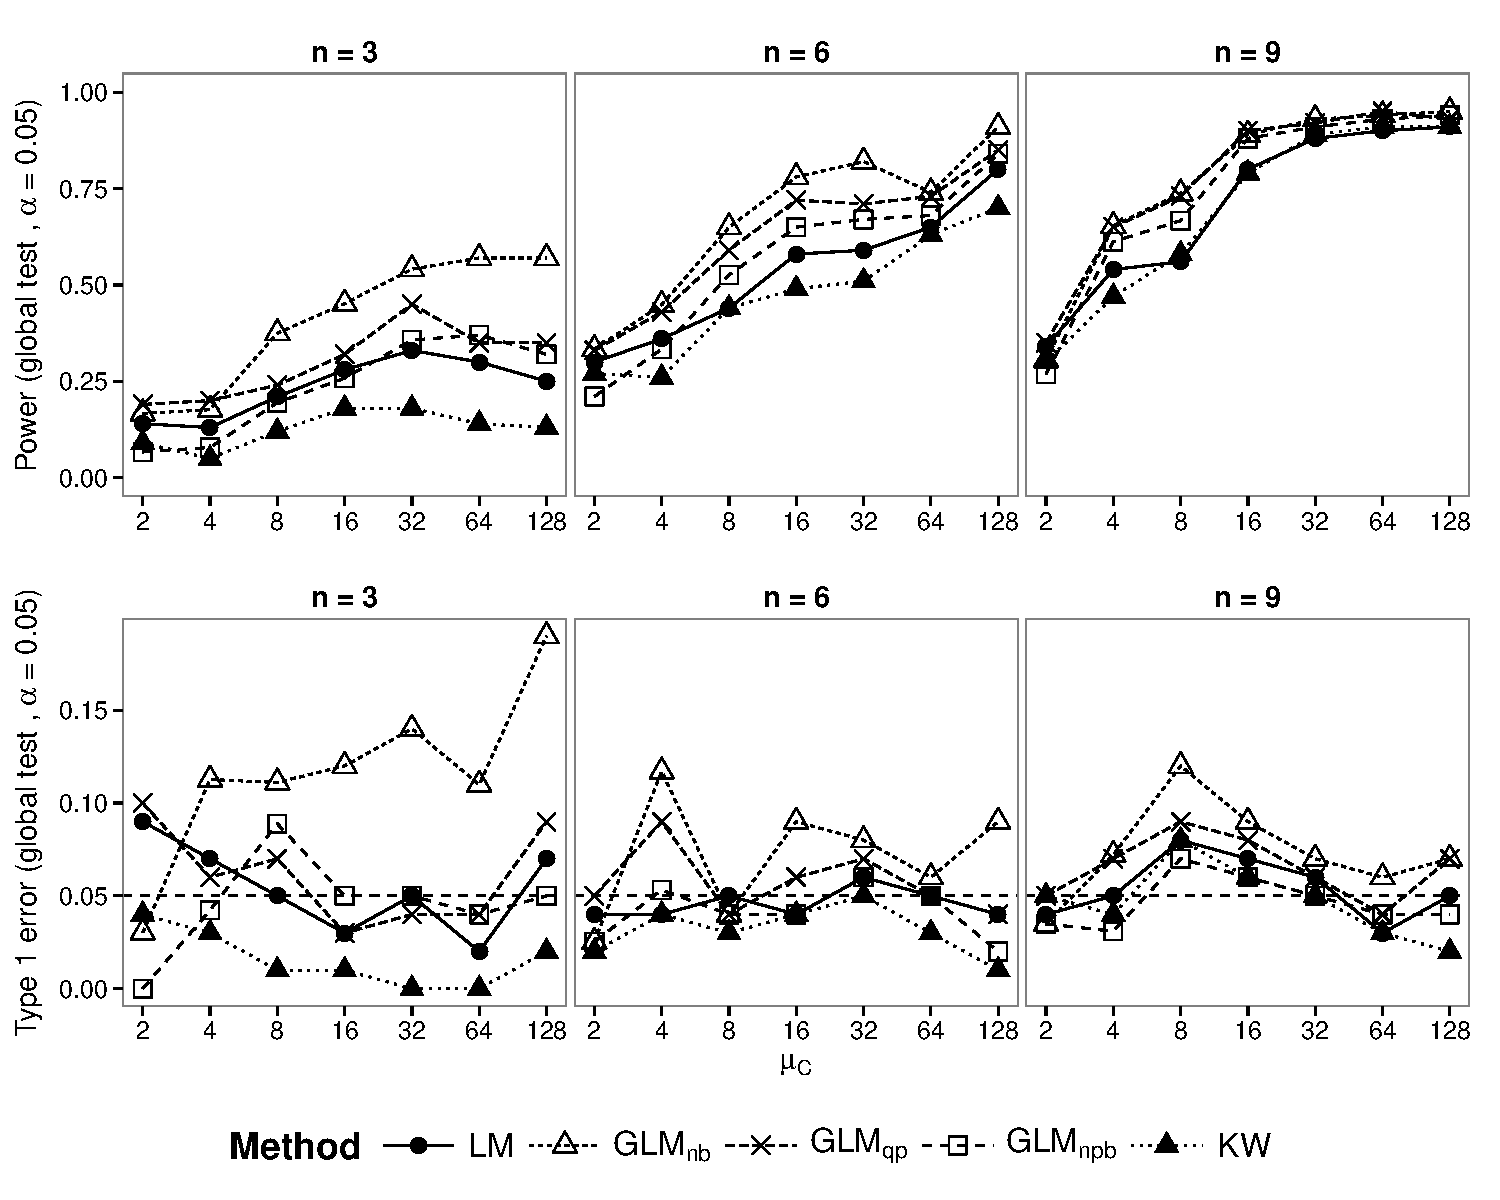
\includegraphics[width = 0.8\textwidth]{p_glob_c.pdf}
  \caption{Simulation results of count data. Power (top) and Type I error (bottom) for the test of a treatment effect.}
  \label{fig:p_glob_c}
\end{figure}

\begin{figure}
  \centering
  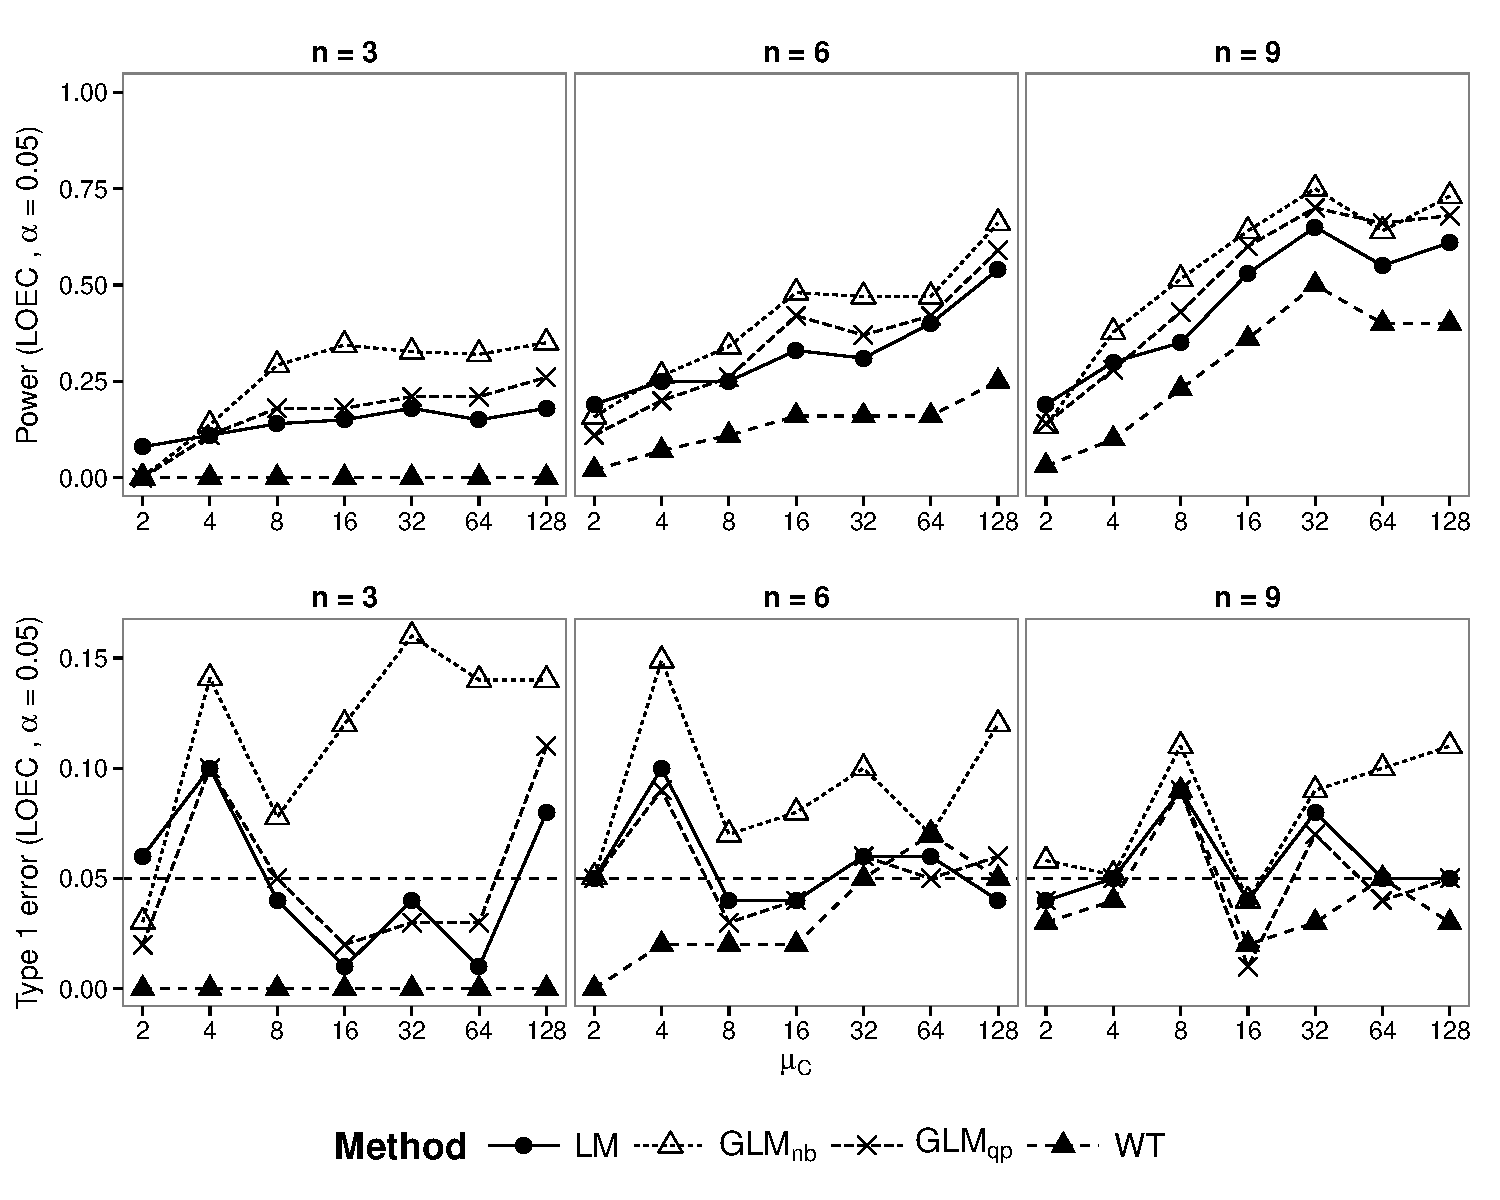
\includegraphics[width = 0.8\textwidth]{p_loec_c.pdf}
  \caption{a}
  \label{fig:p_loec_c}
\end{figure}



\subsection{Binomial data}
\subsubsection{Methods}
We simulated data from a design as described in the motivating example, with 5 treated (T1 - T5) and a control group (C). 
We draw proportion from a Bin(10, $\pi$) distribution, with varying probability of success ($\pi$ = \{0.60, 0.65, 0.70, 0.75, 0.80, 0.85, 0.90, 0.95\}) and varying number of replicates (N = \{3, 6, 9\}).
For Type I error estimation $\pi$ was held constant between groups.
For power estimation $\pi$ in C and T1 was set to 0.95 and $\pi$ in T2-T5 varied between 0.6 and 0.95).

\subsubsection{Results}




\begin{figure}
  \centering
  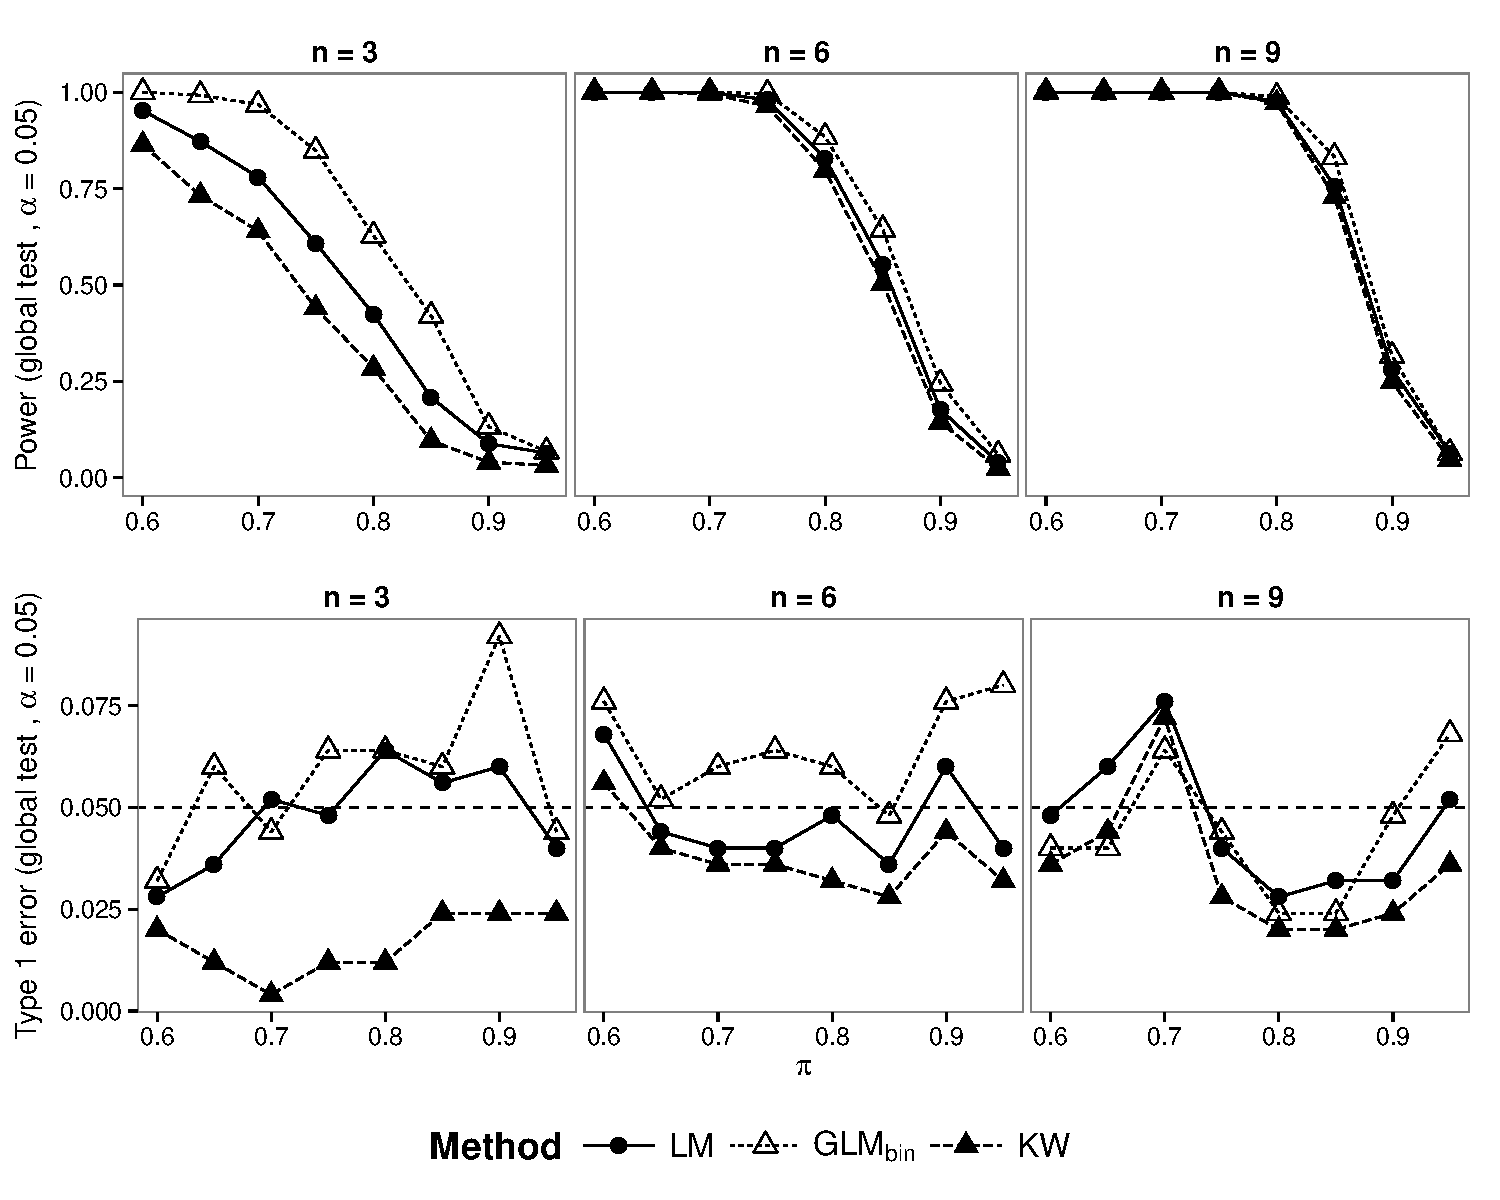
\includegraphics[width = 0.8\textwidth]{p_glob_p.pdf}
  \caption{a}
  \label{fig:p_glob_p}
\end{figure}

\begin{figure}
  \centering
  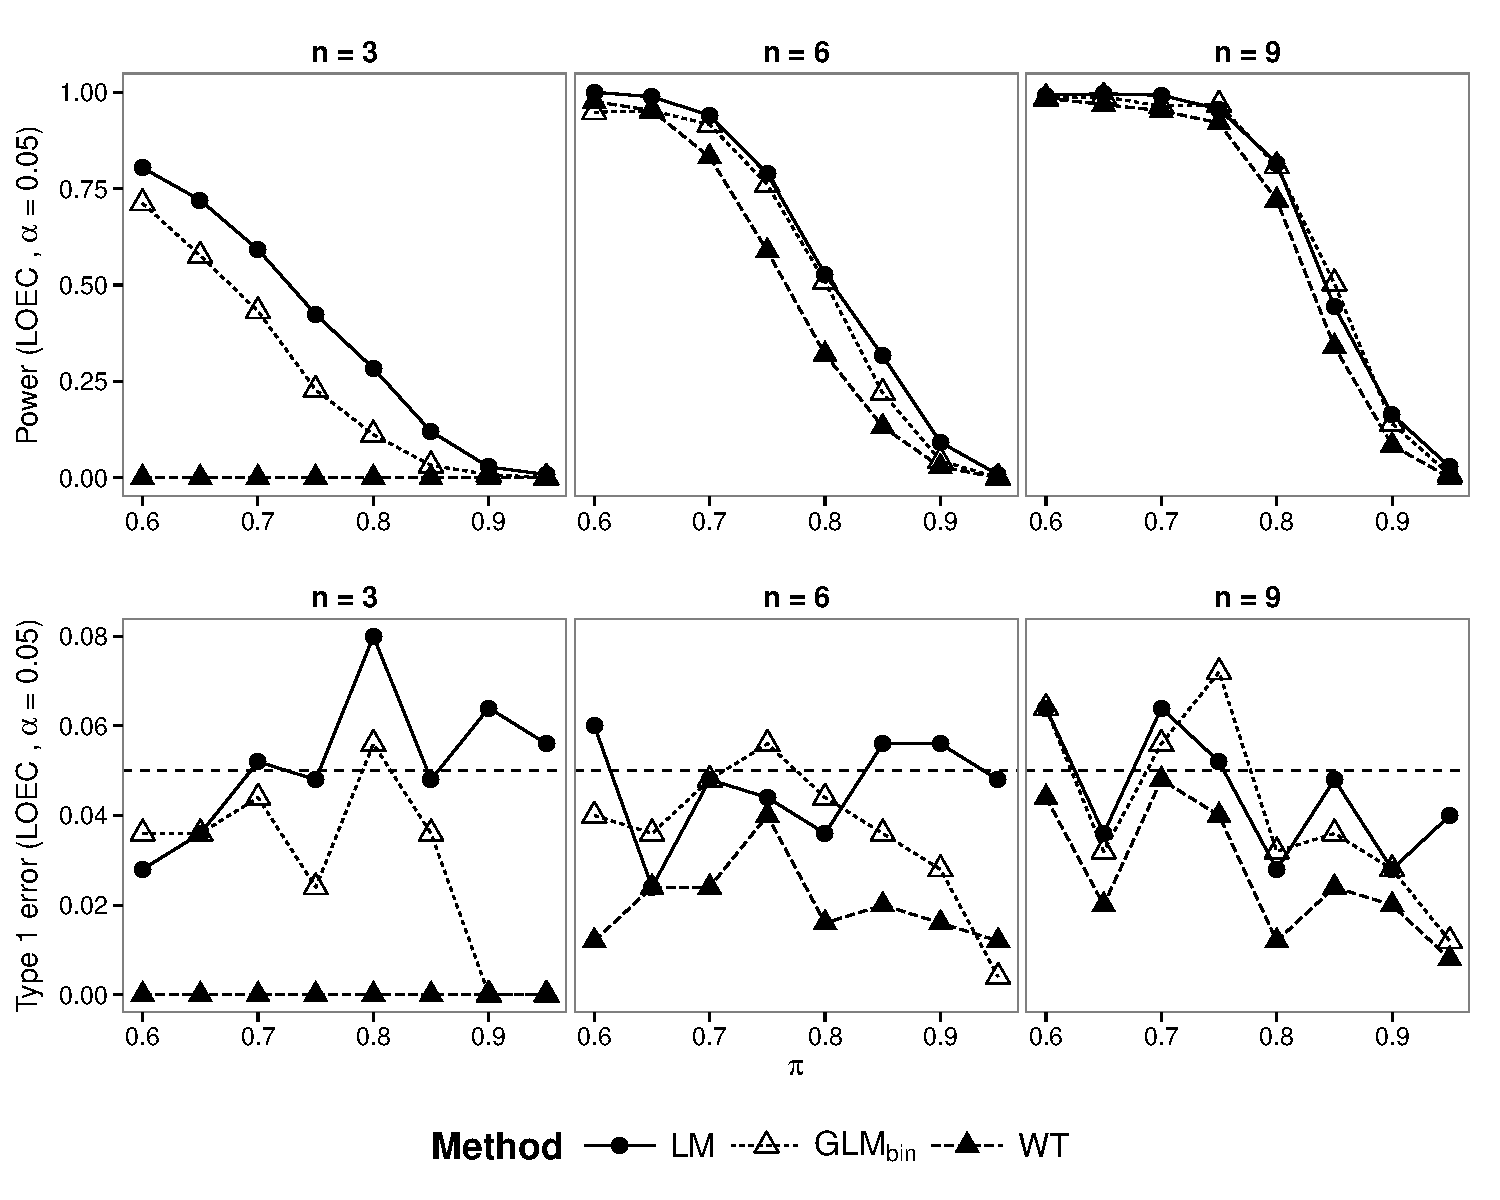
\includegraphics[width = 0.8\textwidth]{p_loec_p.pdf}
  \caption{a}
  \label{fig:p_loec_p}
\end{figure}




\section{Discussion}
\todo{How to choose models? MV plot,...}
\todo{Multivariate}
\todo{GLMM}
\todo{robust SE for lower T1 error in glm nb?}


\section{Conclusions}


\bibliography{references}
\bibliographystyle{apalike}

\end{document}
